\documentclass[12pt,a4paper]{journal}
\usepackage{geometry}

\usepackage{times}

\usepackage[utf8]{inputenc}
\usepackage[T1]{fontenc}
\usepackage{indentfirst}
\usepackage{amsmath}
\usepackage{amsfonts}
\usepackage{amssymb}
\usepackage{caption}
\usepackage{subcaption}
\usepackage{graphicx}
\usepackage{siunitx}
\sisetup{range-phrase=--, range-units=single}

\graphicspath{{img/}}
\usepackage[numbers, super]{natbib}

\begin{document}

\section*{Retinal physiology and therapeutic approaches}

\subsection*{Physiology}

\subsubsection*{In health}

The retina is a layer of tissue less than \SI{0.5}{\mm} thick, that lines the back of the eye.~\cite{Gupta_2015}
The retinal inner surface is attached to the vitreous body, the clear gel that separates the lens and the retina, while its outer surface is attached to Bruch's membrane, see Figure~\ref{fig:architecture-eye}.
When looking at a cross section of the retina as shown in Figure~\ref{fig:architecture-eye}, several layers can be identified, the innermost (closest to the vitreous) being the nerve fiber layer and the outermost the retinal pigmented epithelium (RPE).
Each layer of the retina contains a different type of cells.
The layers located above the RPE are made of neurons and synapses and is referred to as the neurosensory retina.
In the centre of the retina is a oval-shaped pigmented area called the macula that can be seen on photographs of the retina (see Figure~\ref{fig:Scans}).

\begin{figure}[hb]
  \centering
  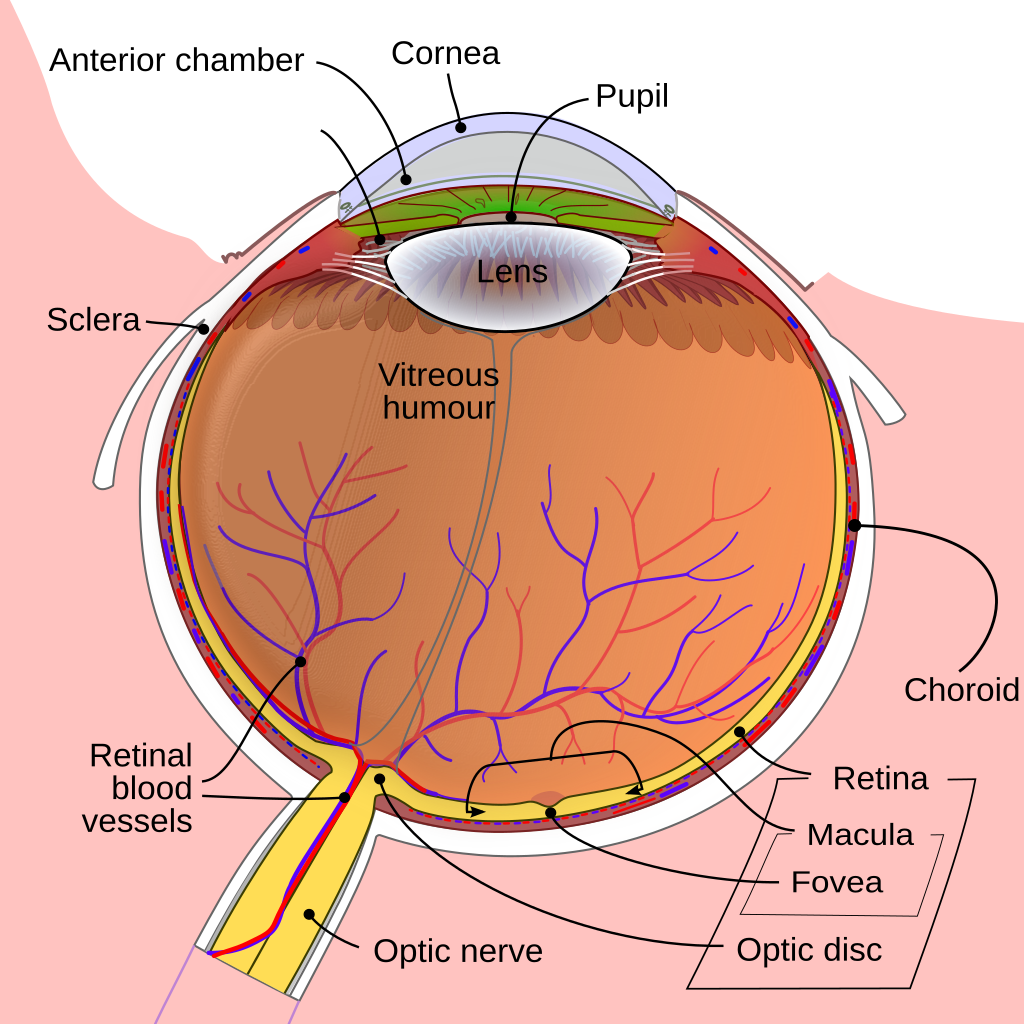
\includegraphics[width=0.45\textwidth, height=7cm]{ArchitectureEye} % From Wikipedia retina
  \hfill
  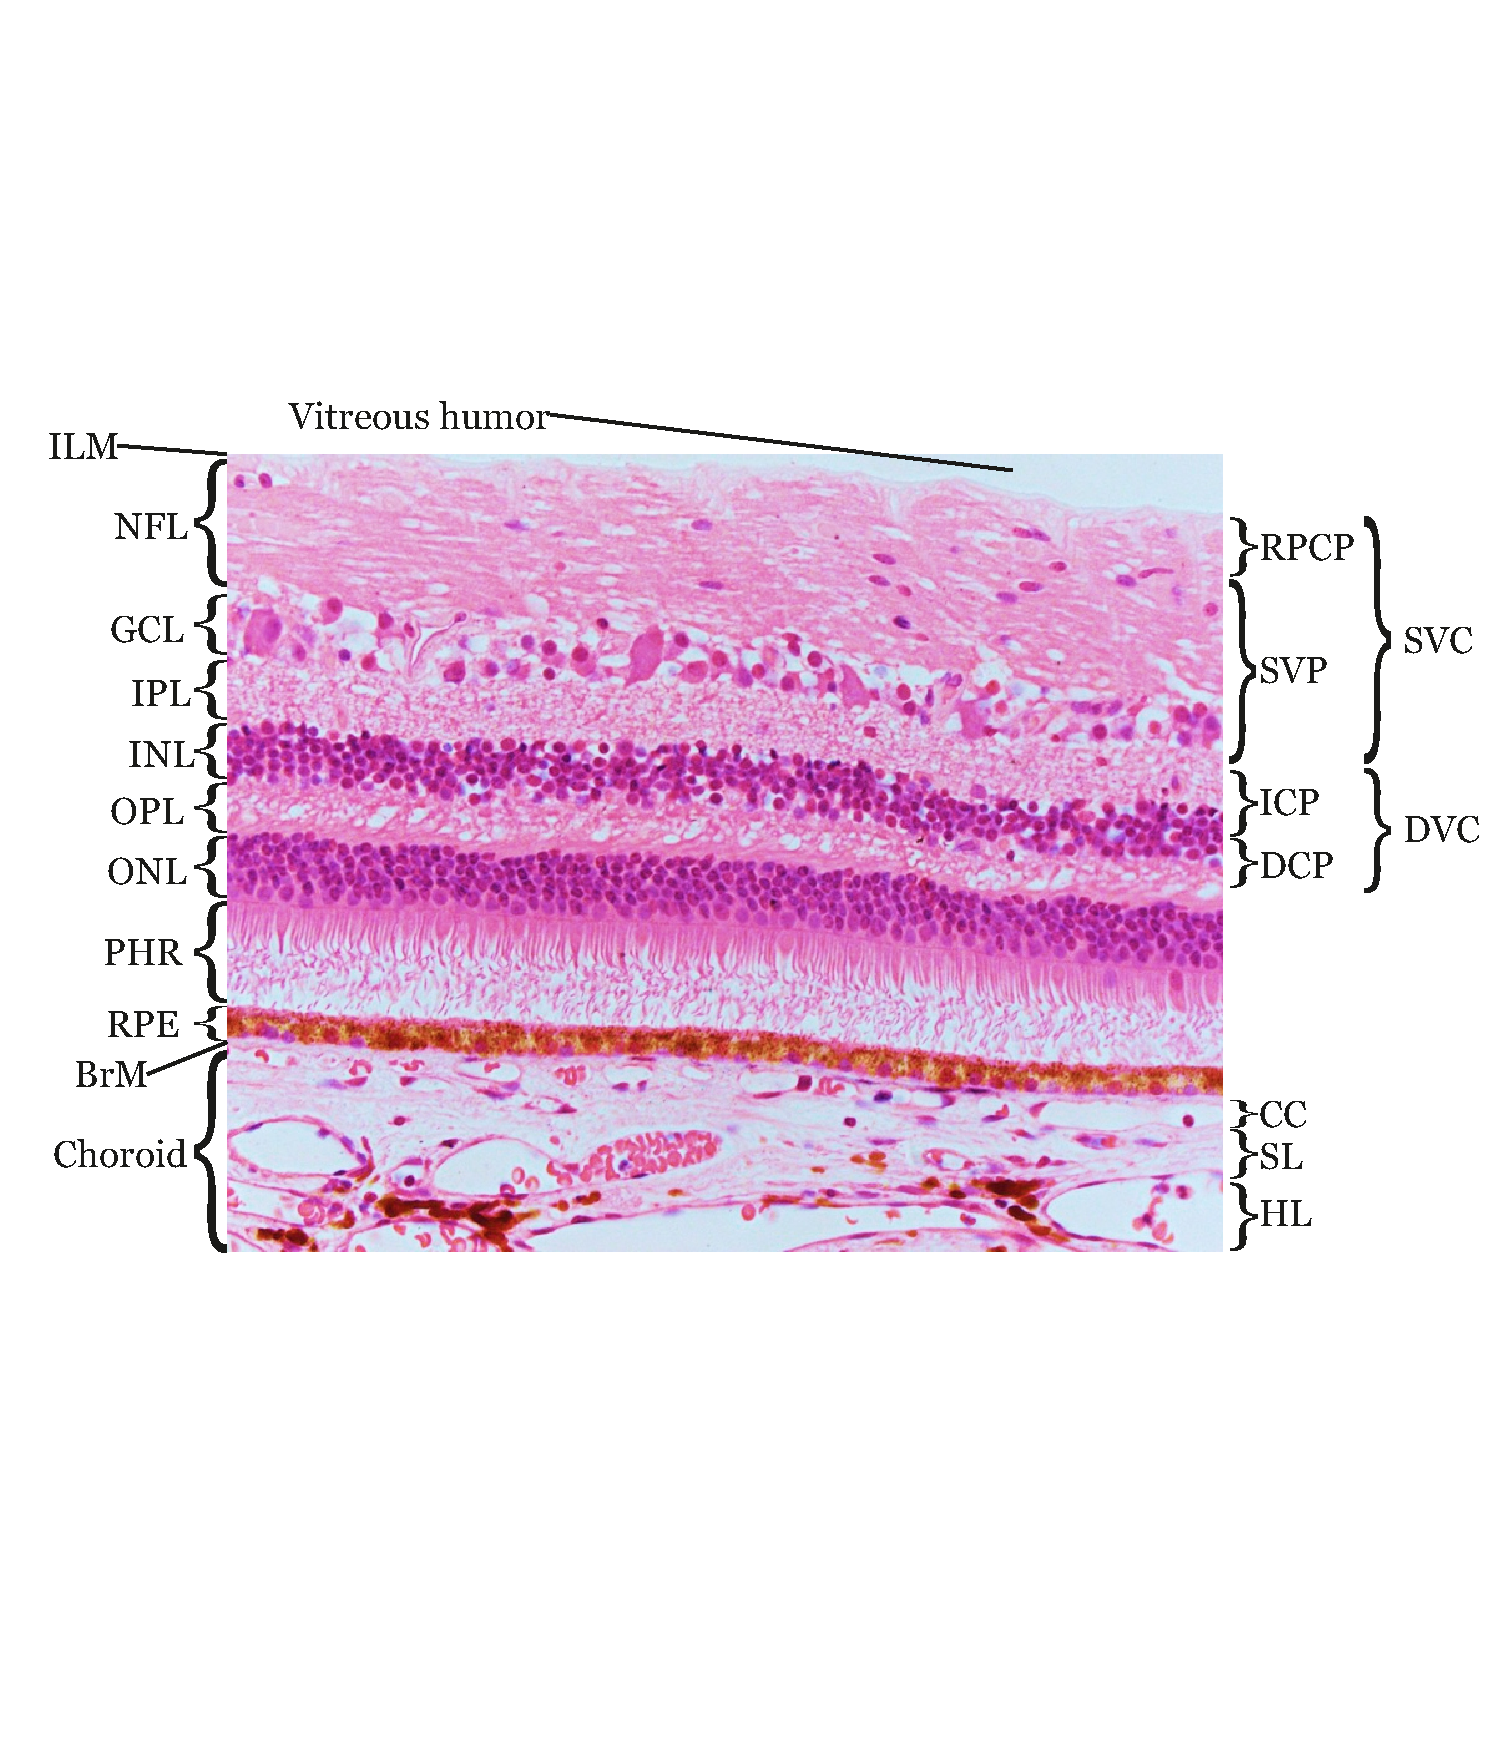
\includegraphics[width=0.5\textwidth, height=7cm]{RetinalLayers2}
  \caption{Anatomy of the eye and the retina. \textbf{(Left)} Anatomy of the eye. Image credits: Rhcastilhos and Jmarchn, CC BY-SA 3.0, via Wikimedia Commons. \textbf{(Right)} The retina and its subdivision in layers. From inner retina to outer retina: inner limiting membrane (ILM), nerve fiber layer (NFL), ganglion cell layer (GCL), inner plexiform layer (IPL), inner nuclear layer (INL), outer plexiform layer (OPL), outer nuclear layer (ONL), photoreceptors (PHR), retinal pigmented epithelium (RPE), Bruch's membrane (BrM), choriocapillaris (CC), Sattler's layer (SL), Haler's layer (HL). Modified from the work of Trivi\~no et al., published under CC BY 3.0 license.~\cite{Trivino_2012}}
  \label{fig:architecture-eye}
\end{figure}

The macula is about \SI{5}{\mm} wide and is responsible for the highly detailed, central vision, owed to its high concentration of photoreceptor cells, namely rods and cones.
In particular, cones are highly concentrated in the centre of the macula, in a pit approximately \SI{1.5}{\mm} wide named the fovea.
The fovea is a critical area of the retina, with a number of conditions appearing at or around it.

Another important structure of the retina in disease is the optic disc.
The optic disc appears as a round spot on fundus photographs of the retina (Figure~\ref{fig:Scans}) and is around \SI{1.8}{\mm} wide.
Through the optic disc passes the optic nerve, the fibers of which extend to form the nerve fiber layer, which transmits visual information to the brain.
The optic nerve is composed of the axons of the retinal ganglion cells, amounting to between $500,000$ and $1.2$ millions, and is surrounded by connective tissue.~\cite{Salazar_2019}

\begin{figure}[ht]
  \centering
  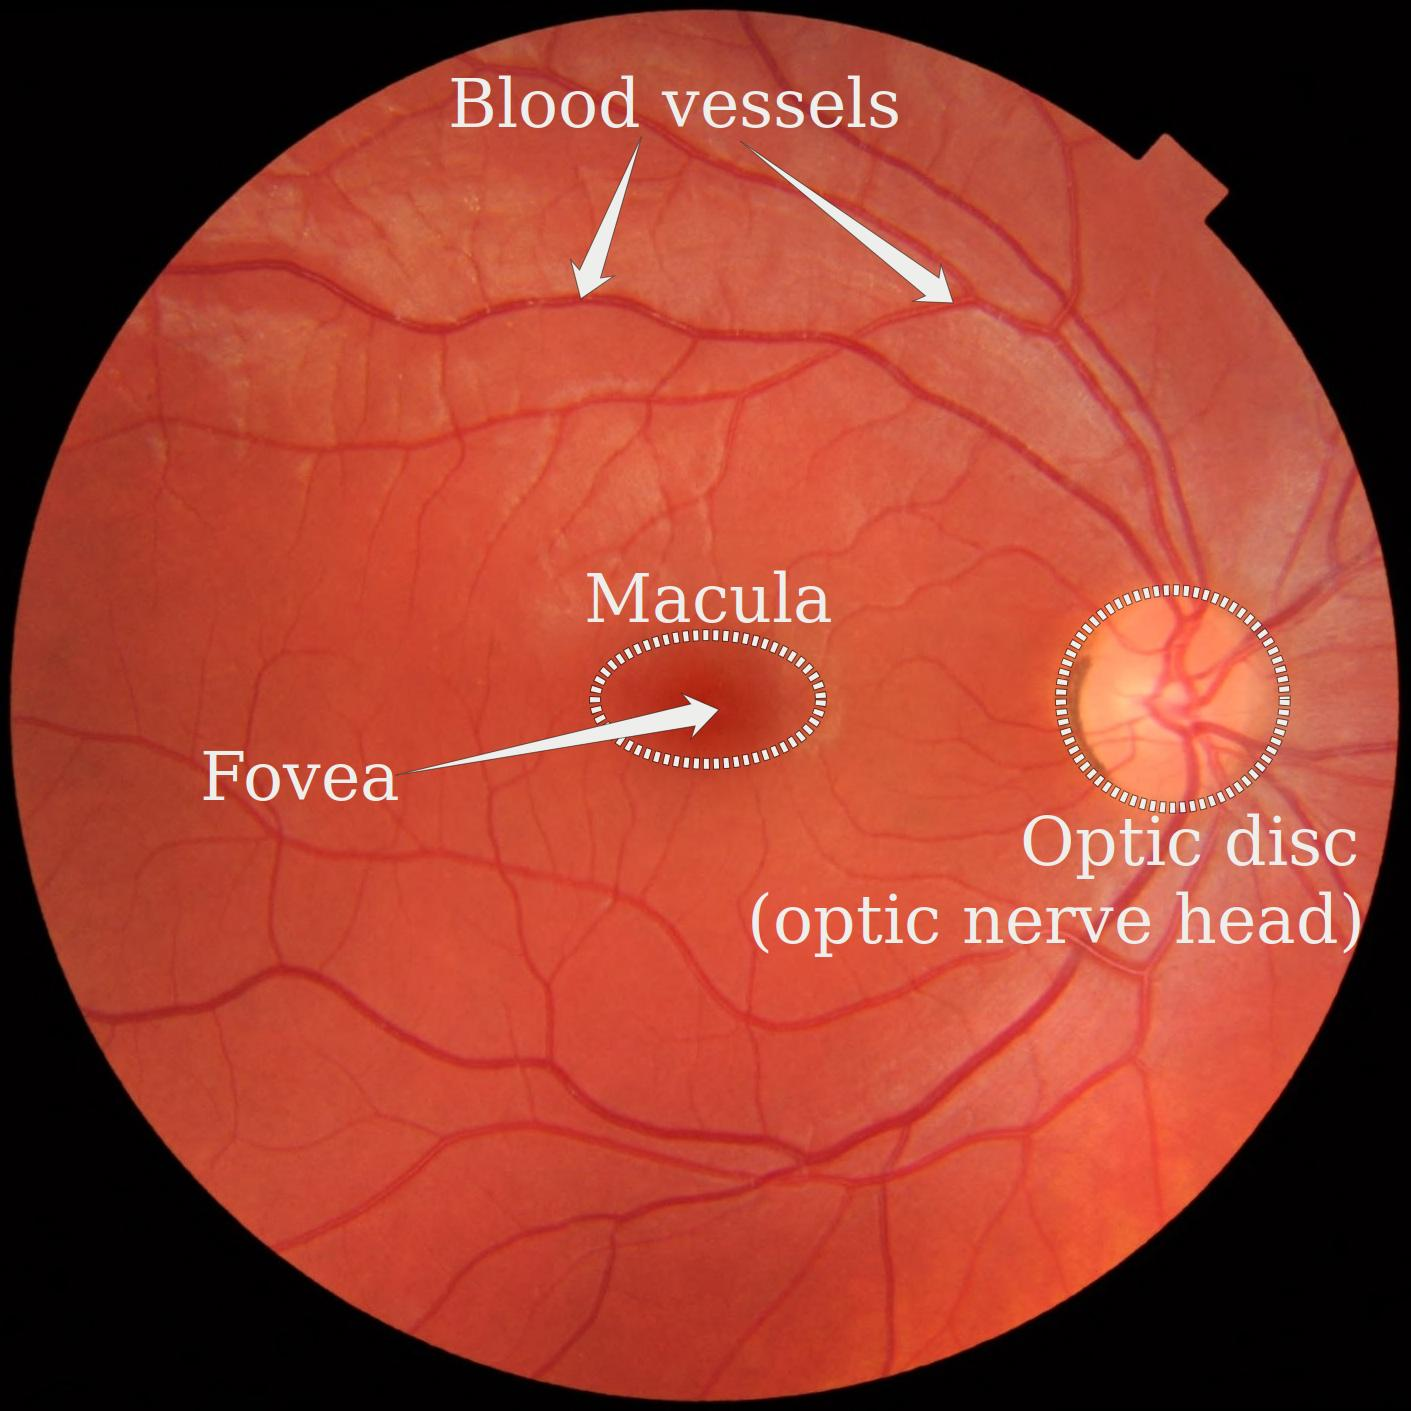
\includegraphics[width=0.45\textwidth]{FA}
  \caption{Anatomical features of the healthy retina on a fundus photograph. By Mikael H\"aggstr\"om, used with permission.}
  \label{fig:Scans}
\end{figure}

Phototransduction, the conversion of light into an electrical signal, results from a cascade of events in the retina. 
Visual information originates from light hitting the retina.
The light crosses the retinal thickness to reach the body of the photoreceptors, in the layer just before the RPE (see Figure~\ref{fig:architecture-eye}).

Activation of photoreceptors by photon starts a cascade of biochemical reactions that transforms light into a biochemical signal.~\cite{Hurley_2009}
This biochemical signal is picked up by cells in the inner layers of the retina, which transform it into an electrical signal.~\cite{Arslan_2018}
The electrical signal is then transmitted to the nerve fiber layer, which relays it to the brain via the optic nerve, enabling vision.

Owing to its pigmentation, the RPE acts as a buffer for remaining lights, protecting the retina from light damage and preventing backreflection of light that may interfere with the visual outcome.
The RPE is formed of a single layer of epithelial cells, which primary function is to support photoreceptors.
To fulfil this purpose, the RPE acts as the blood-retinal barrier, hence regulating the transport of ions, fluid, proteins and other molecules.~\cite{Boulton_2001}
The photoreceptors are attached to the RPE cells' plasma membrane.
Through this close interaction, the RPE collects by-products of the photoreceptors, a washout essential to maintain a healthy neurosensory retina.
The RPE also transports nutrients such as retinoids to the cell where they are essential for the production of the light-sensitive rhodospin protein.~\cite{Boulton_2001} 
Those by-products are released into the systemic circulation via the choroid, one of the two circulations of the retina.~\cite{Boulton_2001}
The cells of the RPE also play a major role in the immune response in the retina and in maintaining the choroidal vasculature through secretion of various vascular growth factors.~\cite{Boulton_2001,Detrick_2020} 

Visual functions require high metabolic activity from the retinal cells, which makes the retinal tissue very demanding in oxygen.
In fact, the rates of oxygen consumption per unit volume of tissue are comparable for the brain and the retina.~\cite{Medrano_1995}
To sustain the demand in oxygen, the retina is equipped with a dense network of capillaries, that branches out of the central retinal artery (CRA) and finishes at the central retinal vein (CRV).
The CRA is a branch of the ophthalmic artery and the CRV drains into the superior ophthalmic vein.
Both the CRA and CRV enter and exit the retina along the optic nerve.
The CRA's branches spread across four plexi within the inner half of the retinal depth, namely, the superficial vascular plexus (SVP) and the intermediate (ICP), deep (DCP) and the radial peripapillary capillary plexus (RPCP).
The terms superficial vascular complex (SVC) and deep vascular complex (DVC) are sometimes used to designate the RPCP-SVP complex and the ICP-DCP complex, respectively.
The inner retinal circulation provides oxygen for the inner \SIrange{60}{80}{\percent} of the tissue.
The perfusion of the remaining outer \SIrange{20}{40}{\percent} is covered by the choroid.

The choroid is a vascular tissue of the eye that lies behind the RPE, from which it is separated by Bruch's membrane.
Bruch's membrane is a thin (\SIrange{2}{4}{\micro\meter}), permeable barrier that provides structural support to the RPE and regulates gas and mass exchanges with the choroid.~\cite{Curcio_2013}
The choroid is structured in three vascular layers.
From the outermost to the innermost: Haller's layer, Sattler's layer and the choriocapillaris (CC).
The diameter of the vessels in each layer decreases as it approaches the retina, with the CC only composed of capillaries.
The vascular input to the choroid is provided by the short posterior ciliary arteries (between 6 and 12), which are branches of the ophthalmic artery.~\cite{Kiel_2010}
The large vessels of the two outer layers of the choroid run parallel to the retinal axis.
Some arterioles from Sattler's layer branch at an almost \SI{90}{\degree} angle to perfuse the CC.~\cite{Nickla_2010}
Each of these arterioles form an hexagonal-shaped domain, fed by a single arteriole and drained by a varying number of venules back into Sattler's layer.~\cite{Zouache_2016}
The capillaries of the CC have wide lumen (the cavity delimited by the vessel's walls), between \SIrange{7}{40}{\micro\meter} in the CC against \SIrange{5}{10}{\micro\meter} in the retina, and are arranged into a single plane, with many connection between adjacent capillaries, also known as anastomosis.~\cite{Bill_1983, ChanLing_2011,Fryczkowski_1994}
Furthermore, the capillary walls have opening (or fenestration), increasing their permeability.~\cite{Nickla_2010}
The fenestrations on the capillary walls are more numerous on the side facing the retina and are at least wide enough to let molecules with a diffusional radius of \SI{3.7}{\micro\meter} pass into the blood.~\cite{Nickla_2010, Bill_1983}
This particular architecture combined with a high blood flow allows the CC to provide enough oxygen through diffusion across Bruch's membrane and the RPE and to clear wastes from the retina through the systemic circulation.

The blood supply from the choroid to the outer retina is indirect.
Therefore, the choroid has high blood flow and a high oxygen content.~\cite{Bill_1983}
The high concentration of oxygen in the choroidal circulation creates a strong gradient for its diffusion between the choriocapillaris and the outer retina.
The high blood flow rates may also help regulating the temperature of the macula, by keeping it at the same temperature as the rest of the body.~\cite{Bill_1983, Parver_1991}

While appropriate blood supply is necessary to maintain vision, blood vessels can interfere with light and hinder resulting images.
The distribution of photoreceptor in the retina is heterogeneous, with a higher concentration in the parafovea, for rods, and fovea, for cones.~\cite{Zouache_2022}
For this reason, the centre of the fovea is an avascular zone around \SI{500}{\micro\meter} wide, often referred to as the foveolar avascular zone (FAZ).

The interactions between layers of the retina, e.g., the RPE and photoreceptors, is essential to visual functions.
Disruption of the delicate structure of the retina leads to degeneration of sight.

\subsubsection*{In disease}

% A number of different retinal pathologies can lead to loss of sight.
% Loss of sight can be caused by direct loss of the photoreceptors, such as in age-related macular degeneration (AMD), retinitis pigmentosa and diabetic retinopathy.~\cite{Gupta_2015, Birch_1999}
% This loss may be secondary to a loss of the balance in supply demand of oxygen.
% Causes include degeneration of the retinal or choroidal circulation, Bruch's membrane and the RPE.

% However, conditions affecting the nerve, blocking the transmission of visual signal to the brain are also very common.
% For example, glaucoma is a degeneration of the optic nerve and the nerve fiber layer caused by an increase in the pressure generated by the fluids in the vitreous, namely the intraocular pressure.~\cite{Quigley_2011}

While the retina is a key element of visual functions, its relative fragility makes it susceptible to a number of conditions, some of which may lead to blindness.
Loss of visual acuity can be caused by failures at any level of the phototransduction cascade.\\
\textbf{Dry age-related macular degeneration.}
The dry form of age-related macular degeneration (AMD) is a common condition in individuals over fifty years of age.
It is characterised by the presence of accumulated cellular debris under (drusen) and above (reticular pseudo-drusen) the RPE.~\cite{Bottos_2012}
The drusen and pseudo-drusen appear when accumulated stress from age and other environmental factors such as cigarette smoking and diet cause the dysfunction of the RPE's clearance functions.
In the end-stage of dry AMD, RPE cells degenerate and form geographic atrophy in the macula.~\cite{Jager_2008}
Geographic atrophy is the name given to patches of atrophied RPE cells that can be seen on fundus photographs.
Ultimately sight loss is due to the atrophy of the photoreceptors deprived from the support of underlying RPE cells, but a gradual distortion of images is also present from the early stages.~\cite{Newsom_2008,Zacks_2022}\\
\textbf{Retinitis pigmentosa.}
Similarly, individuals with retinitis pigmentosa (PR) progressively lose sight from degeneration of the photoreceptors.
Disease-related mutations are typically expressed by rods, leading to their degeneration in early stages of PR.
For a reason still unclear, cones cells degeneration follows from the absence of rods, despite cones not expressing the mutations responsible for rods death.
Multiple hypothesis have been suggested for this phenomenon.
One of them is the oxygen toxicity hypothesis.
As the choroid lacks the capacity to regulate blood flow accordingly to metabolic needs of the retina, some suggested that the absence of rods leads to high oxygen tension in the photoreceptor layers, an hyperoxia detrimental to cones survival.~\cite{Roberts_2018,Stone_1999}
Another hypothesis speculates that cones survival is dependent on a trophic factor provided by rods.
Therefore, the later degeneration of cones could be explain by the absence of such factor.~\cite{Roberts_2022}\\
\textbf{Diabetic retinopathy.}
One of the consequences of diabetes is the degeneration of the smaller vessels in the retina, the capillaries.
Such degeneration include an increase in vascular permeability, a loss of the pericytes coating capillary walls and a thickening of the endothelial basement membrane upon which endothelial cells are attached.~\cite{Medina_2016}
Additionally, a rarefaction of capillaries can be observed around the foveal avascular zone.
Such microvascular degeneration's may cause microvascular occlusions, haemorrhages and oedemas as well as macular ischaemia.~\cite{Medina_2016}
The subsequent release of vascular endothelial growth factor (VEGF) may progress the diabetic retinopathy (DR) to its proliferative stage.
In proliferative DR, elevated VEGF levels cause the growth of abnormal capillary membranes in a process known as neovascularization.
The neovascular membranes cause further haemorrhages and oedemas and scaring of the tissue.
Scaring and the toxicity of blood damage the photoreceptors, sometimes permanently, resulting in dramatic loss of sight.~\cite{Friedlander_2007,Gupta_2015}
Moreover, the neovasculature may pierce through the inner limiting membrane and haemorrhage in the vitreous or preretinal space, the potential space between the inner limiting membrane and the vitreous, disturbing vision.\\
\textbf{Neovascular age-related macular degeneration}
The neovascular form of AMD is characterised by a much more dramatic loss of sight and the appearance of macular neovasculature (MNV).
As most cases of neovascular AMD happen in eyes affected by dry AMD, it may be referred to as a late stage of AMD.
The current understanding of the pathogenesis of neovascular AMD is that, in addition to other age-related changes in the retina, the progressive buildup of materials in Bruch's membrane characteristic of dry AMD induces hypoxic conditions in the outer retina.~\cite{Jager_2008,Newsom_2008}
The subsequent upregulation of VEGF by RPE cells stimulate angiogenesis in the choriocapillaris.~\cite{Jager_2008}
The resulting neovasculature may pierce through Bruch's membrane, growing below the RPE, or through the RPE, growing in between the RPE and the photoreceptors, in the subretinal space.
The neovasculature may also emerge from the inner retinal circulation.
Regardless of the location, neovascular membranes are associated with oedema, haemorrhage, scarring and RPE or retinal detachment (when the retina separating from the RPE), all of which cause the quick loss of sight observed in neovascular AMD.~\cite{Gupta_2015,Jager_2008}\\
\textbf{Retinal tears and breaks}
Tears may occur in the retina for various reasons, including trauma and surgery.
Posterior vitreous detachment is another reason for the apparition of tears and breaks (tears through the whole thickness of the neurosensory retina).
With age, the vitreous humor undergoes progressive liquefaction.
In addition, there is gradual loss of adhesion between the inner limiting membrane and the posterior vitreous cortex to which it is attached.~\cite{Bottos_2012,Medina_2016}.
The combination of those two factors facilitates the accumulation of vitreous fluid in the preretinal space, tearing apart the inner limiting membrane and the vitreous.
However, in areas of strong adhesion of the inner limiting membrane, the mechanical forces induced by the fluids can cause retinal tears or breaks and macular holes.~\cite{Shechtman_2009}
Macular holes cause blurry vision while retinal tears provide a path to the subretinal space which may fill with fluids, causing retinal detachment.~\cite{Medina_2016}
Additionally, the traction caused by the fluid in the preretinal space can cause retinal detachment.\\
\textbf{Retinal vessel occlusion}
A number of conditions may cause blood vessel in the retina to clog or collapse.
Accumulation of plaque caused by, for example, cholesterol, or a blood clot (embolus) in blood vessels form an obstruction to blood flow.~\cite{Medina_2016}
Sickle cell retinopathy causes a stiffening of red blood cells which can result in occlusion of arterioles or capillaries, but also of the central retinal artery.~\cite{Medina_2016}
Mechanical pressures such as ocular hypertension can cause the collapse of veins, including the central retinal vein, when the external pressure becomes higher than the blood pressure.~\cite{Hayreh_2004}
Stiffening of the central retinal artery is suspected to also compress the central retinal vein.~\cite{Medina_2016}
Occlusion of arteries causes non-perfusion areas in the retina, stopping visual functions in the affected areas.
Irreversible damage to the retina starts appearing after \SI{100}{\min} of non-perfusion.~\cite{Hayreh_2004}
Some patients with retinal vein occlusion may develop retinal ischaemia, though the reasons are unclear.~\cite{Khayat_2018}
Other symptoms include retinal oedema and, in some cases, neovascularization in various locations, including the optic disc and the retina.~\cite{Medina_2016}
\\
\textbf{Glaucoma}
Glaucoma is a group of optic neuropathies affecting the optic nerve and the ganglion cell layer of the retina (see Figure~\ref{fig:architecture-eye}).
Ophthalmologist observe a thinning of the ganglion cell layer and degeneration of the tissue of the optic nerve.
Those symptoms are due to degeneration of the ganglion cell bodies (in the ganglion cell layer) and axons (forming the optic nerve).~\cite{Quigley_2011}
it is thought that a combination of ocular hypertension and changes in cerebrospinal fluid pressure and retinal blood pressure create a pressure gradient around the optic nerve, increasing mechanical stresses on the tissue.~\cite{Band_2009,Nickells_2012}
Vision loss in glaucoma is due to the loss of connectivity between the retina and the brain and cannot be recovered.~\cite{Quigley_2011} 


\subsection*{Therapeutic strategies}

\subsubsection*{Surgeries}

Retinal detachment often requires emergency surgery to preserve vision.
Different methods are available to reconnect the retina with the RPE.
One possibility is to insert a so-called scleral buckle in the sclera, the white tissue supporting the eyeball and located behind the choroid in the retina.
The scleral buckle will push the sclera towards the detached retina.~\cite{Sodhi_2008}
Another approach consist in pushing the retina towards the RPE.
This technique named pneumatic retinopexi consist in injecting a gas bubble into the vitreous~\cite{Sodhi_2008}.
The tension created by the gas pushes the retina back into contact with the RPE.
Once contact is restored, the RPE can drain the liquid that accumulated in the retinal holes.
The gas is naturally removed from the vitreous. 
In more complicated cases of retinal detachment, e.g., in the presence of vitreous haemorrhage, vitrectomy might be preferred to pneumatic retinopexi.
Vitrectomy consist in replacing the vitreous humour with either a silicone oil substitute or a gas bubble, favourising reattachment in a similar fashion as pneumatic retinopexi.~\cite{Dervenis_2022}
Surgeries for retinal detachment may also be complemented with ILM peeling, cryotherapy or laser photocoagulation.
Because the ILM contributes to retinal rigidity and in vitreal traction of the retina, its removal may be useful to facilitate closure of retinal holes and lower the rate of reopening after surgery.~\cite{Chatziralli_2018}
Cryotherapy and photocoagulation can be performed to scar the tissue around retinal tears, effectively sealing them to prevent spread that may lead to retinal detachment.
Cryotherapy and photocoagulation can be used alone or after pneumatic retinopexi or vitrectomy.~\cite{Sodhi_2008}

Photocoagulation may also be used to address abnormal neovasculature in diabetic retinopathy or vessel occlusion.~\cite{Evans_2014}
The burn induced by the laser therapy to the retinal tissue is aimed to stop further vascular growth by either sealing or ablating the aberrant blood vessels (focal laser photocoagulation) or by ablating in a wider range (panretinal laser treatment).
In the case of panretinal laser treatment, it is thought that the damage brought to the retinal tissue causes a change in the oxygen supply and demand balance that could lower VEGF expression.~\cite{Evans_2014}
Photodynamic therapy is a similar approach which uses photochemical mechanisms to induce cell death rather than heat which may be preferred for destroying neovasculature in the more fragile foveal region, for example in eyes with neovascular age-related macular degeneration.~\cite{SchmidtErfurth_2000}

In eyes with glaucoma, the aim of surgery is to lower intraocular pressure.
This can be done by decreasing the pressure in the aqueous chamber.~\cite{Quigley_2011}
Laser treatment of the trabecular meshwork, an area of tissue around the base of the cornea (Figure~\ref{fig:architecture-eye}), is aimed to improve drainage of the aqueous humor.
In some cases, parts of the trabecular meshwork may be removed to allow further drainage in a procedure called trabeculectomy.
Conversely, intraocular pressure can be lowered by decreasing the production of aqueous humor, acting on the inflow rather than the outflow of aqueous humor.
This treatment, referred to as cyclodiode therapy, aims to reduce this inflow by destroying the ciliary body that produces aqueous humor.~\cite{Allbon_2022}

\subsubsection*{Drug based}

The regulation of intraocular pressure can be achieve with drugs.
In fact most patients with glaucoma begin treatment with eye-drops, used daily to reduce intraocular pressure.
The eye-drops are designed to lower the aqueous humor production, increase drainage of aqueous humor, or both.~\cite{Chakrabarti_2022,Quigley_2011}

Retinal vascular disorders such as neovascular age-related macular degeneration, proliferative diabetic retinopathy or retinal vein occlusion, are for the most part treated with anti vascular growth factors (VEGF).~\cite{Andreoli_2007,Kim_2021}
These drugs, mostly injected in the vitreous humor, bind to VEGF molecules that drive the growth of immature and leaky blood vessels.
Anti-VEGF treatment has proven effective to suppress disease progression, reducing retinal oedema and restoring vision.~\cite{Andreoli_2007,Heier_2006,Kim_2021}
Steroids, either oral or intravitreal, can also be prescribed to reduce the production of pro-inflammatory cytokines such as VEGF in order to increase the RPE functions in patients with retinitis pigmentosa presenting macula oedema.~\cite{Strong_2016}

Deterioration of visual functions due to ageing (cellular senescence), whether normal or fasten by disease, has been addressed by a range of therapeutics called senotherapeutics.
Their use for the is being investigated as a mean to maintain vision in disease such non-neovascular age-related macular degeneration which lack therapeutic targets.~\cite{Lee_2021}


\subsubsection*{Other}

Alternative intervention types are possible, however, their use remain rare as they are investigated for efficiency and safety.
Retinal prosthesis have started being approved for use in late stage of certain retinal diseases such as retinitis pigmentosa.~\cite{Luo_2016}
The artificial retina replaces the degenerated photoreceptors by a video camera.~\cite{Luo_2016,Stingl_2017}
The pixelated image is then transferred to the inner retina's neurons, relatively spared by retinitis pigmentosa, using microelectrodes.
The transfer of the electrical signal to the brain is then achieved normally through the optic nerve.~\cite{Luo_2016,Stingl_2017}

Because matured RPE and photoreceptor cells are unable to divide and proliferate, stem cell therapy is a promising therapeutic approaches in eyes with photoreceptor or RPE atrophy such as age-related macular degeneration.~\cite{Berta_2011,Stern_2015}
Stem cells are naturally found in the body and have yet to form into a specific cell type and have the ability to form into many different cell types.
Therefore, stem cells injected into the retina are able to replace degenerated RPE or photoreceptor cells and halt loss of vision or even improve vision.~\cite{ONeill_2020}

Gene therapy is an intervention that aims to slow the progress of inherited retinal diseases such as retinitis pigmentosa.
It consists in introducing copies of healthy genes into the retina in order to reduce degeneration from disease-related mutations.~\cite{Battu_2022}
Viruses are designed to safely deliver the healthy genes to cells, which will either replace or silence the mutant genes.~\cite{Battu_2022} 


% % \begin{spacing}{0.0}
% \bibliographystyle{abbrvnat} % {ksfh_nat}
% {\normalsize \bibliography{section_2}}
% % \end{spacing}

\end{document}
